\documentclass[12pt]{exam}

% \usetikzlibrary{calc,patterns}

\newcommand{\Version}{1} 
\newcommand{\Solutions}{0} 

% TEST SPECIFIC INFORMATION
\ifnum \Version=1 \newcommand{\TestName}{MATH 2552 Participation Activity 7: Numerical Methods} \fi


% LOAD PACKAGES
\usepackage{amsmath} % allows for align env and other things
\usepackage{amssymb} % 
\usepackage{mathtools} % allows for single apostrophe
\usepackage{enumitem} % allows for alpha lettering in enumerated lists
\usepackage{lastpage}
\usepackage{array} % for table alignments

\usepackage{graphicx} % if images are needed
\usepackage{wrapfig} % to allow text wrapping

\addpoints

\usepackage{pgfplots} % for surfaces (chapter 7)
\usepackage{tikz-3dplot} 
\pgfplotsset{compat=1.9}
\usetikzlibrary{decorations.pathmorphing,patterns} % for some tikz diagrams
% ~~~~~~~~~~~~~~~~~~~~~~~~~~~~~~~~~~~~
% INITIALS
\newcommand{\Initials}{\textit{\Course, \TestName. Your initials: \underline{\hspace{3cm}}} \vspace{1pt}}

\newcommand{\InitialsLeft}{\noindent \hspace{-18pt}\textit{\Course, \TestName. Your initials: \underline{\hspace{3cm}}} \vspace{1pt}}

\newcommand{\InitialsRight}{\begin{flushright}\textit{\Course, \TestName. Your initials: \underline{\hspace{3cm}}} \vspace{1pt}\end{flushright}}

% ADJUST FIRST LINE IN PARAGRAPH INDENTATION 
\setlength\parindent{0pt}

% FONT FORMAT
\renewcommand*\rmdefault{lmss} % change font to lat mod ss

% ADJUST MARGINS 
\usepackage[a4paper, tmargin=0.8in,bmargin=0.8in,left=1in,right=1in]{geometry}

% TIKZ DIAGRAMS
\usepackage{color}
\usepackage{tikz}  \usetikzlibrary{arrows} 
\usetikzlibrary{calc} 

% COURSE SPECIFIC INFORMATION
\newcommand{\Course}{Math 2552, Differential Equations}
\newcommand{\Instructors}{}

\newcommand{\LastPage}{\begin{center}\textit{This page may be used for scratch work. Please indicate clearly if you would like your work on this page to be graded. }\end{center}   }

% DERIVATIVES
\newcommand{\dfdy}{{\frac{df}{dy}}} % 
\newcommand{\dydt}{{\frac{dy}{dt}}} % 
\newcommand{\dxdt}{{\frac{dx}{dt}}} % 
\newcommand{\dydx}{{\frac{dy}{dx}}} % 
\newcommand{\dydtt}{{\frac{d ^2y}{dt^2}}} % 
\newcommand{\dydxx}{{\frac{d^2y}{dx^2}}} % 
\newcommand{\dydttt}{{\frac{d^3y}{dt^3}}} % 

\newcommand{\ddt}{{\frac{d}{dt}}} % 
\newcommand{\ddx}{{\frac{d}{dx}}} % 
\newcommand{\ddy}{{\frac{d}{dy}}} % 
\newcommand{\dudt}{{\frac{du}{dt}}} % 
\newcommand{\dvdx}{{\frac{dv}{dx}}} % 
\newcommand{\dxdtt}{{\frac{d^2x}{dt^2}}} % 
\newcommand{\dzdt}{{\frac{dz}{dt}}} % 

% COLORS FOR SOLUTIONS
\definecolor{DarkBlue}{rgb}{0.0,0.2,0.4} % 
\definecolor{DarkRed}{rgb}{0.4,0.1,0.1} % 
\definecolor{DarkGreen}{rgb}{0.0,0.25,0.15} % 

% % ADJUST MARGINS
% \usepackage[tmargin=2.0in,bmargin=1.5in]{geometry}
% \geometry{margin=0.76in}

% ADJUST FIRST LINE IN PARAGRAPH INDENTATION 
\setlength\parindent{0pt}

% FONT FORMAT
\renewcommand*\rmdefault{lmss} % change font to lat mod ss


% HEADERS AND FOOTERS
\pagestyle{headandfoot}
\runningfooter{}{}{}
\runningheader{}{}{\textit{\TestName, Page \thepage \ of \pageref{LastPage}} }
% \headheight 42pt % distance from top of page to top of header
% \headsep 12pt % space between header and top of body


\begin{document}
    
\vspace*{-1cm}

\begin{center}
{\Large \TestName}
\end{center}
\newcommand{\ID}{Please print your first name: \framebox{\strut\hspace{4.2cm}}, last name: \framebox{\strut\hspace{4.2cm}}, \\[2pt] and the remaining digits of your GTID:  \framebox{\strut $9$}\framebox{\strut $0$}\framebox{\strut\hspace{0.19cm}}\framebox{\strut\hspace{0.19cm}}\framebox{\strut\hspace{0.19cm}}\framebox{\strut\hspace{0.19cm}}\framebox{\strut\hspace{0.19cm}}\framebox{\strut\hspace{0.19cm}}\framebox{\strut\hspace{0.19cm}}.}

\ID

\vspace{6pt}
\textbf{Instructions}: for full credit please show your work and answer all questions. Your work will be graded for completion, not accuracy. Please submit your work before the end of lecture. 

\subsection*{Exercises}
\begin{questions}

\question[3] Consider the following IVP: $\displaystyle \dydt + y + t/2 = 0, \ y(0) = 1, \ t \ge 0$. The exact solution is $y(t) = \frac12 ( 1 - t + e^{-t})$. A graph of $y$ is shown below. 
        \begin{center}
        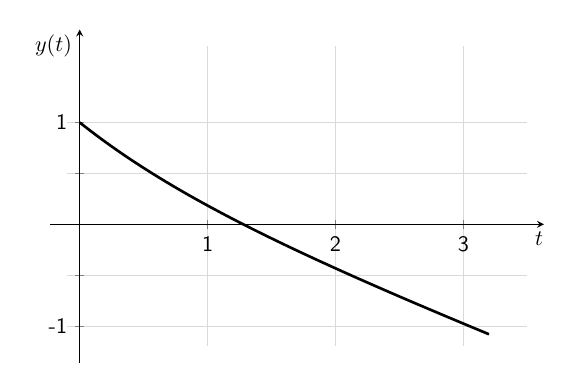
\begin{tikzpicture}[scale=.8] 
            \begin{axis}[
            width=3.5in,
            height=2.5in,
            clip=false,
            axis lines=middle,
            xmin=-.1,xmax=3.5,
            ymin=-1.2, ymax=1.75,
            xtick={1,2,3},
            xticklabels={1,2,3},
            ytick={-1,-0.5,0,0.5,1},
            yticklabels={-1,,0,,1},        
            axis line style={shorten >=-7.5pt, shorten <=-7.5pt},
            xlabel=$t$,
            ylabel=$y(t)$,
            xlabel style={at={(ticklabel* cs:1)},anchor=north west},
            ylabel style={at={(ticklabel* cs:1)},anchor= east},
            grid style={line width=.4pt, draw=gray!30},
            grid=both,
            ]
            \addplot[black,samples=501,domain=0:3.2,very thick] {0.5 - x/2 +.5*exp(-x)};% 
            \end{axis}
        \end{tikzpicture} 
        \end{center}      
\begin{parts}
    \part Construct the equation of the tangent line to $y(t)$ at $t=0$. Use your tangent line to estimate $y(t)$ at $t=1$. Add the tangent line to the graph above. \vfill
    \part We can get a better estimate of $y(1)$ by using two steps. Use the Euler method with step size $h=0.5$ to estimate $y(1)$. \vfill
    \newpage
    \part Now use a spreadsheet or other software to estimate $y(1)$ with step size $h=0.1$ and $h = 0.01$. What are your estimates? 
    \vspace{2cm}
\end{parts}

\question[1] The IVP below models the two-compartment fluid tank we saw earlier in the course. 
\begin{align}
    \dxdt = \frac12(y-x) , \quad \dydt = \frac12 (x-y), \quad x(0)=3, \quad y(0) = 1
\end{align}
The exact solution is given by
\begin{align}
    x(t) &= 2 + e^{-t} \\
    y(t) &= 2 - e^{-t}
\end{align}
Use a spreadsheet or other software to estimate $x(1)$ and $y(1)$ with step size $h=0.1$ and $h = 0.01$. What are your estimates? 

\begin{itemize}
    \item When $h=0.1$, $x(1) \approx$ \vspace{12pt}
    \item When $h=0.1$, $y(1) \approx$ \vspace{12pt}
    \item When $h=0.01$, $x(1) \approx$ \vspace{12pt}
    \item When $h=0.01$, $y(1) \approx$
\end{itemize}
\end{questions}

\end{document}




\documentclass[12pt]{exam}

% \usetikzlibrary{calc,patterns}

\newcommand{\Version}{1} 
\newcommand{\Solutions}{0} 

% TEST SPECIFIC INFORMATION
\ifnum \Version=1 \newcommand{\TestName}{MATH 2552 Participation Activity 7: Numerical Methods} \fi


% LOAD PACKAGES
\usepackage{amsmath} % allows for align env and other things
\usepackage{amssymb} % 
\usepackage{mathtools} % allows for single apostrophe
\usepackage{enumitem} % allows for alpha lettering in enumerated lists
\usepackage{lastpage}
\usepackage{array} % for table alignments

\usepackage{graphicx} % if images are needed
\usepackage{wrapfig} % to allow text wrapping

\addpoints

\usepackage{pgfplots} % for surfaces (chapter 7)
\usepackage{tikz-3dplot} 
\pgfplotsset{compat=1.9}
\usetikzlibrary{decorations.pathmorphing,patterns} % for some tikz diagrams
% ~~~~~~~~~~~~~~~~~~~~~~~~~~~~~~~~~~~~
% INITIALS
\newcommand{\Initials}{\textit{\Course, \TestName. Your initials: \underline{\hspace{3cm}}} \vspace{1pt}}

\newcommand{\InitialsLeft}{\noindent \hspace{-18pt}\textit{\Course, \TestName. Your initials: \underline{\hspace{3cm}}} \vspace{1pt}}

\newcommand{\InitialsRight}{\begin{flushright}\textit{\Course, \TestName. Your initials: \underline{\hspace{3cm}}} \vspace{1pt}\end{flushright}}

% ADJUST FIRST LINE IN PARAGRAPH INDENTATION 
\setlength\parindent{0pt}

% FONT FORMAT
\renewcommand*\rmdefault{lmss} % change font to lat mod ss

% ADJUST MARGINS 
\usepackage[a4paper, tmargin=0.8in,bmargin=0.8in,left=1in,right=1in]{geometry}

% TIKZ DIAGRAMS
\usepackage{color}
\usepackage{tikz}  \usetikzlibrary{arrows} 
\usetikzlibrary{calc} 

% COURSE SPECIFIC INFORMATION
\newcommand{\Course}{Math 2552, Differential Equations}
\newcommand{\Instructors}{}

\newcommand{\LastPage}{\begin{center}\textit{This page may be used for scratch work. Please indicate clearly if you would like your work on this page to be graded. }\end{center}   }

% DERIVATIVES
\newcommand{\dfdy}{{\frac{df}{dy}}} % 
\newcommand{\dydt}{{\frac{dy}{dt}}} % 
\newcommand{\dxdt}{{\frac{dx}{dt}}} % 
\newcommand{\dydx}{{\frac{dy}{dx}}} % 
\newcommand{\dydtt}{{\frac{d ^2y}{dt^2}}} % 
\newcommand{\dydxx}{{\frac{d^2y}{dx^2}}} % 
\newcommand{\dydttt}{{\frac{d^3y}{dt^3}}} % 

\newcommand{\ddt}{{\frac{d}{dt}}} % 
\newcommand{\ddx}{{\frac{d}{dx}}} % 
\newcommand{\ddy}{{\frac{d}{dy}}} % 
\newcommand{\dudt}{{\frac{du}{dt}}} % 
\newcommand{\dvdx}{{\frac{dv}{dx}}} % 
\newcommand{\dxdtt}{{\frac{d^2x}{dt^2}}} % 
\newcommand{\dzdt}{{\frac{dz}{dt}}} % 

% COLORS FOR SOLUTIONS
\definecolor{DarkBlue}{rgb}{0.0,0.2,0.4} % 
\definecolor{DarkRed}{rgb}{0.4,0.1,0.1} % 
\definecolor{DarkGreen}{rgb}{0.0,0.25,0.15} % 

% % ADJUST MARGINS
% \usepackage[tmargin=2.0in,bmargin=1.5in]{geometry}
% \geometry{margin=0.76in}

% ADJUST FIRST LINE IN PARAGRAPH INDENTATION 
\setlength\parindent{0pt}

% FONT FORMAT
\renewcommand*\rmdefault{lmss} % change font to lat mod ss


% HEADERS AND FOOTERS
\pagestyle{headandfoot}
\runningfooter{}{}{}
\runningheader{}{}{\textit{\TestName, Page \thepage \ of \pageref{LastPage}} }
% \headheight 42pt % distance from top of page to top of header
% \headsep 12pt % space between header and top of body


\begin{document}
    
\vspace*{-1cm}

\begin{center}
{\Large \TestName}
\end{center}
\newcommand{\ID}{Please print your first name: \framebox{\strut\hspace{4.2cm}}, last name: \framebox{\strut\hspace{4.2cm}}, \\[2pt] and the remaining digits of your GTID:  \framebox{\strut $9$}\framebox{\strut $0$}\framebox{\strut\hspace{0.19cm}}\framebox{\strut\hspace{0.19cm}}\framebox{\strut\hspace{0.19cm}}\framebox{\strut\hspace{0.19cm}}\framebox{\strut\hspace{0.19cm}}\framebox{\strut\hspace{0.19cm}}\framebox{\strut\hspace{0.19cm}}.}

\ID

\vspace{6pt}
\textbf{Instructions}: for full credit please show your work and answer all questions. Your work will be graded for completion, not accuracy. Please submit your work before the end of lecture. 
\subsection*{Humans vs. Zombies}

The imagined conflict between humans and zombies has lead to the development of numerous engaging stories, movies, television series, and games. For example, in 2005, a group of Goucher College students invented the game Humans versus Zombies that is also a game on the GT campus. Versions of their game have spread to campuses all over the United States, including at GT! Our approach to modelling Human/Zombie interactions will be to employ the population models we have studied and approximate their solutions with numerical methods. In this activity we assume that zombies are (imaginary) creatures that prey on humans,  that zombies can convert humans to zombies, and that when zombies die they are removed from the population. 

\subsection*{Exercises}
\begin{questions}

\question[5] A model for the populations of zombies $Z(t)$ and humans $H(t)$ could be 
\begin{align}
    H'(t) = k_hH -\alpha Z , \qquad Z'(t) = \alpha Z, \quad H(0) = 1000, \quad Z(0) = 1, \quad \alpha > 0, \quad k_h > 0 
\end{align}
Although simple, this model allows us to develop a numerical method for approximating a solution to an IVP. 
\begin{parts}
    \part Construct the equation of the tangent line to $Z(t)$ at $t=0$ for $\alpha=2$. Use your tangent line to estimate the zombie population at $t=1$. \vfill
    \part Construct the equation of the tangent line at $t=1$. Use this tangent line and your estimate of $Z(1)$ to calculate an estimate of $Z(2)$. \vfill
    \newpage 
    \part Repeat this process to estimate $Z(10)$. You will want to use software to make your calculations more efficient. Based on your calculations, $Z(10) = $ 
    \part What is the exact solution to the DE for $Z(t)$ at $t=10$? \vspace{24pt}
    \part What can you do to improve the accuracy of your calculations? \vspace{24pt}
\end{parts}

\question[3] A model for approximating $H(t)$ and $Z(t)$ that more closely reflects the stated assumptions is to use a predator-prey model that we explored last week in lecture. Using the notation for our problem the predator-prey model has equations:
\begin{align}
    \frac{dH}{dt} = k_hH -\alpha HZ, \qquad \frac{dZ}{dt} = \alpha HZ - k_zZ, \quad H(0) = 4, \quad Z(0) = 1
\end{align}
where $H$ and $Z$ are the populations of humans and zombies measured in thousands.
\begin{parts}
    \part Using $\alpha = 2$, and $k_h=1$, $k_z=4$, estimate the populations of $H$ and $Z$ at time $t=5$. 
    \vspace{2cm}
    \part Give a rough sketch of the populations of $H$ and $Z$ over $0\le t \le 10$. 
\vfill

        \part Why might the predator-prey system in (2) be a more useful model than the system in (1)? \vspace{24pt}
    \vfill
\end{parts}

\end{questions}

\end{document}




